\documentclass{article}
\usepackage[utf8]{inputenc}
\usepackage[polish]{babel}
\usepackage[T1]{fontenc}
\usepackage{listings}

\title{Ultradźwiękowy miernik odległości}
\author{Krzysztof Pakaszewski\\Piotr Seemann\\Wiktor Mendalka\\Numer zespołu: 36\\Informatyka II rok EAIiIB 2018/2019}
\date{Czerwiec 2019}

\usepackage{natbib}
\usepackage{graphicx}

\begin{document}

\maketitle

\section{Schemat}
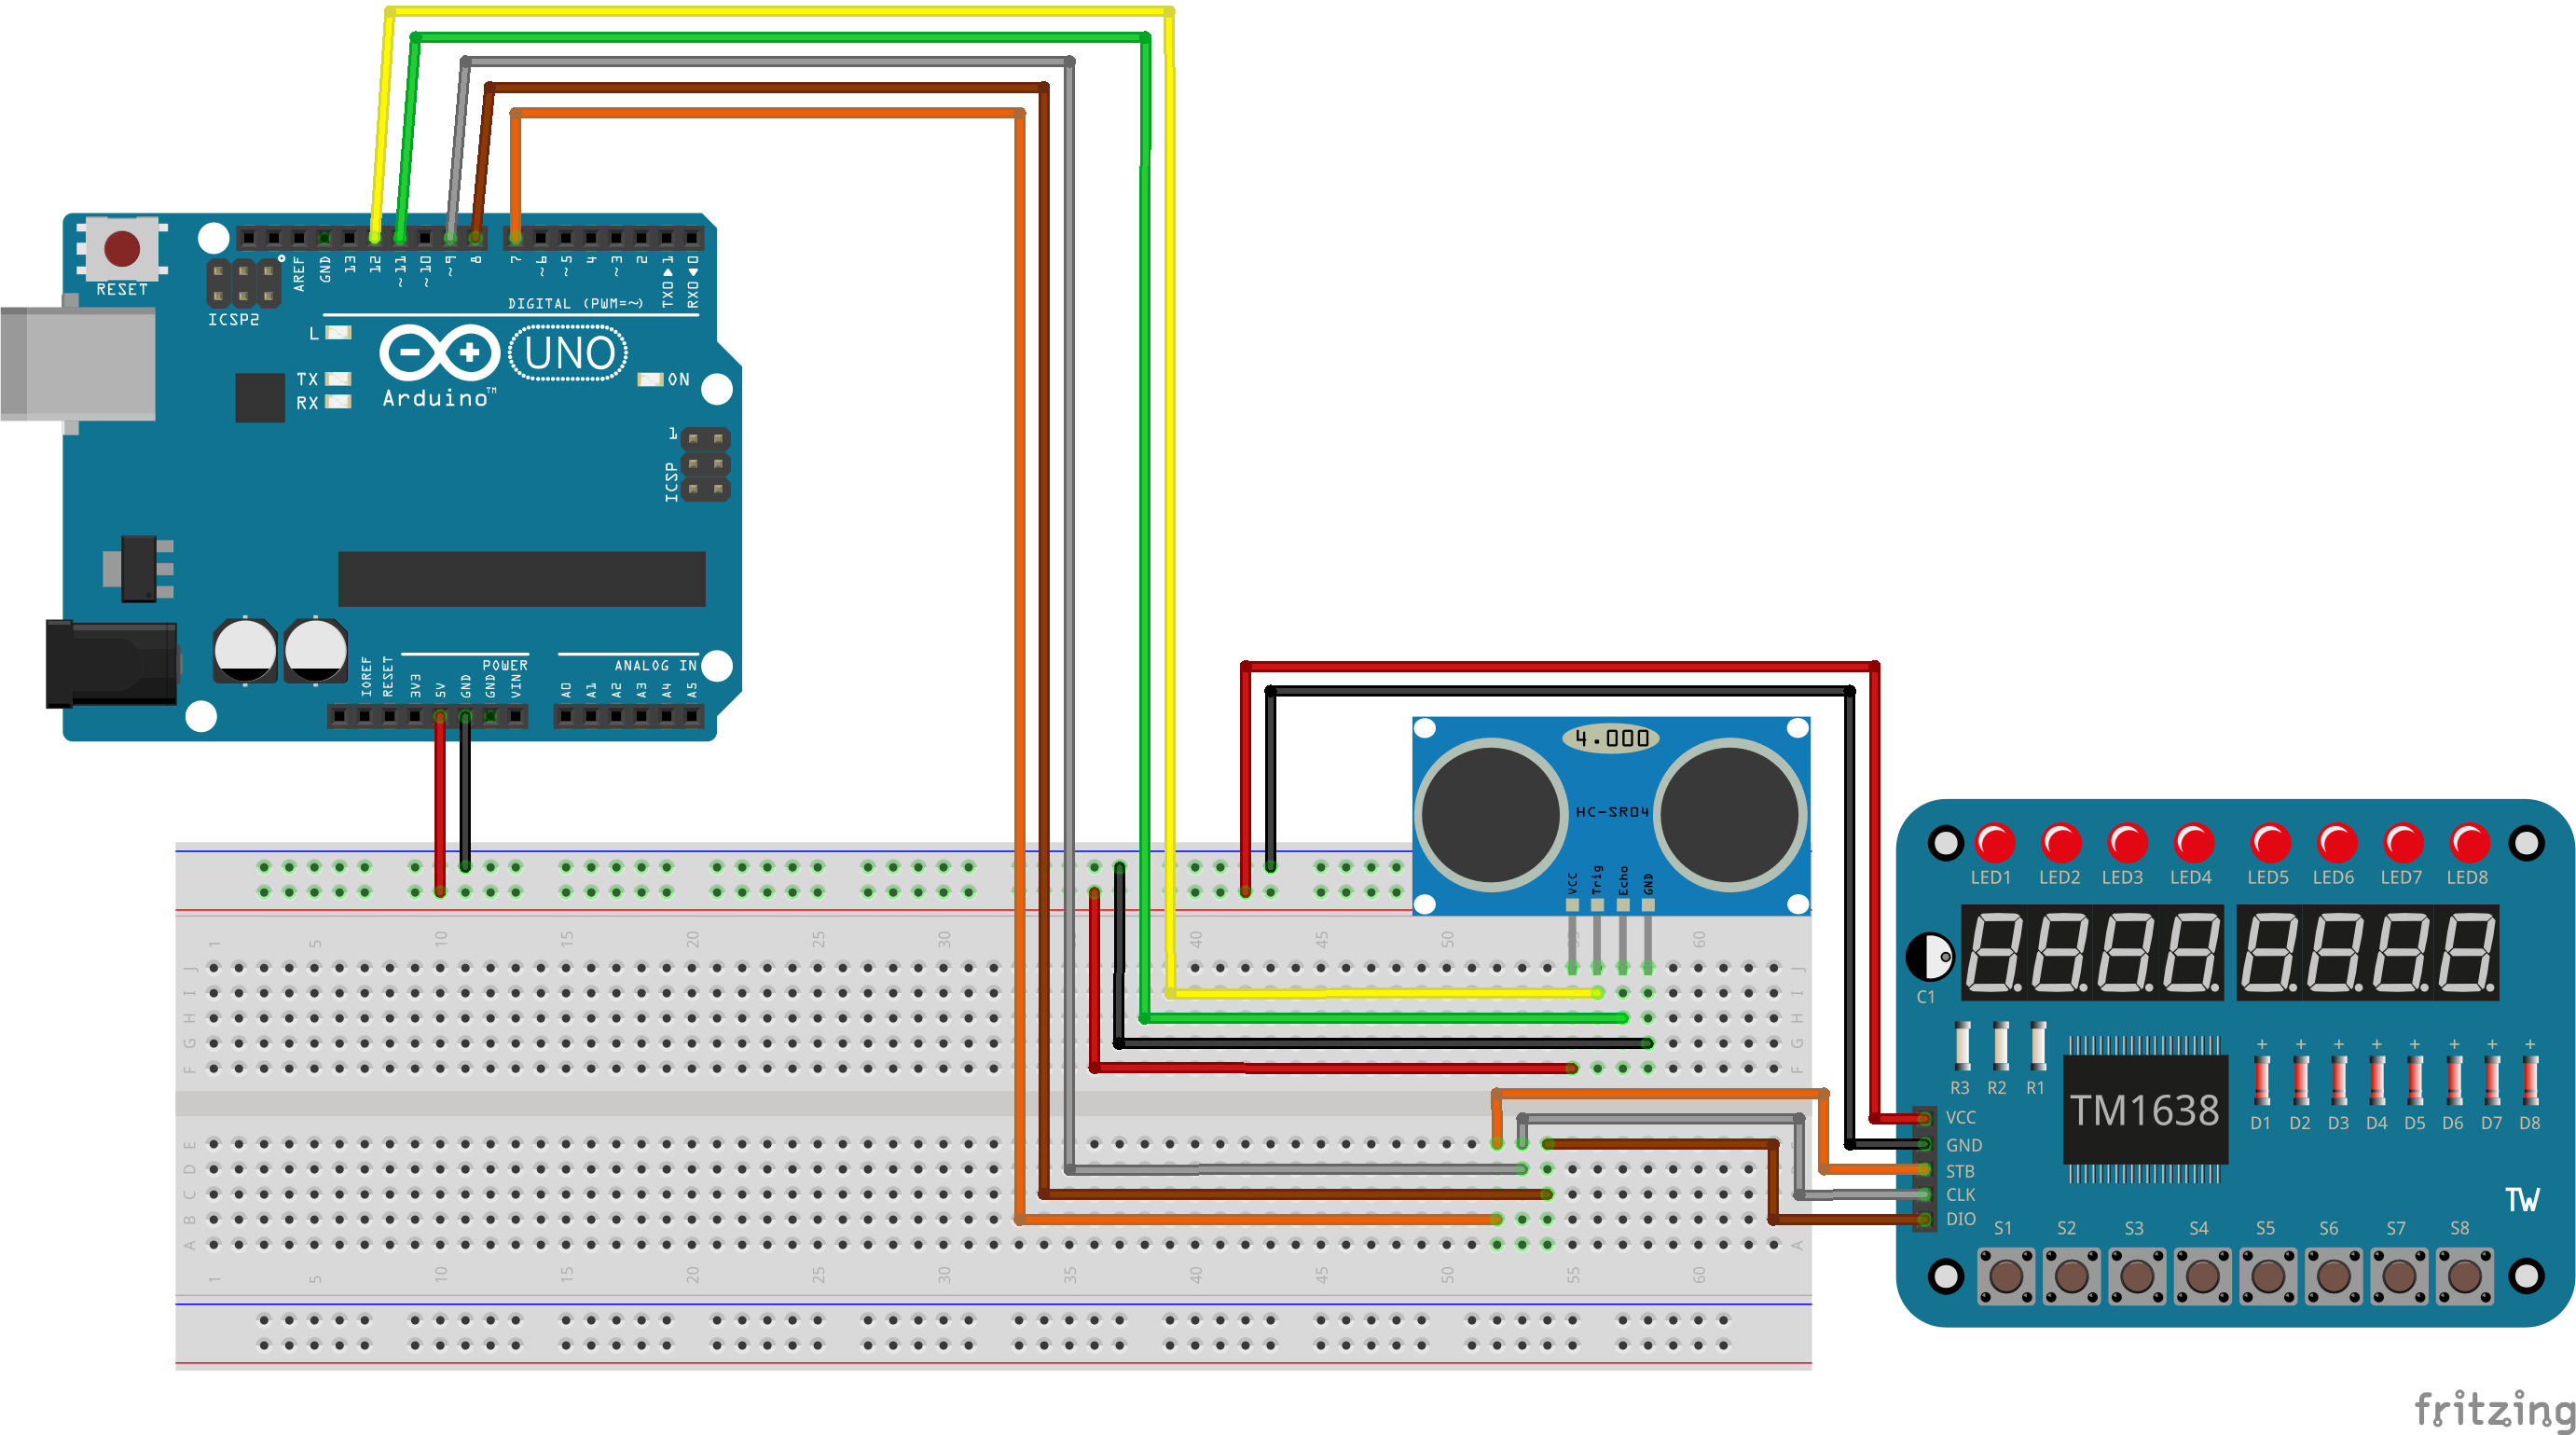
\includegraphics[scale=0.5]{sketch_bb.png}

\section{Opis algorytmu}

Lista kroków:
 \begin{enumerate}
    \item Zacznij algorytm.
    \item Wyświetl migający napis w postaci ‘--------‘ (osiem kresek poziomych).
    \item Po naciśnięciu przycisku S1 wygaś wyświetlacz.
    \item Dokonaj 50 pomiarów czasu biegu fali dźwiękowej do przeszkody i z powrotem, następnie podziel wynik przez 2, żeby otrzymać czas biegu fali do przeszkody i oblicz odległość od przeszkody mnożąc wynik przez prędkość dźwięku ($distance = \frac{duration \cdot 0.034}{2}$).
    \item Oblicz średni dystans.
    \item Wyświetl końcowy wynik pomiaru w formacie xxx.x
    \item Po naciśnięciu przycisku S2 skasuj wynik i powróć do punktu 2.
    \item Zakończ algorytm.
\end{enumerate}

Algorytm działa poprawnie dla zakresu  30-200 cm.


\section{Opis programu}

Zmienne:
 \begin{enumerate}
 	\item digits - jest to tablica, która po odowołaniu się do niej za pomocą cyfry i, zwraca binarny zapis na wymagane dla wyświetlenia tej cyfry LEDy
 	\item dist - przechowuje obliczony dystans
 	\item strobe, clock, data, trigPin, echoPin - wartości stałe przechowujące kody pinów, w które wpięte są przewody
 	\item showValue, test - zmienne pomocnicze pozwalające zachowywać stan wyświetlania, tj. zmieniają wartość, gdy wciśnięte zostaną przeciski mające zmienić tryb pracy
 \end{enumerate}

Metody:
 \begin{enumerate}
 	\item sendCommand - wysyła podaną wartość na strobe, wartość to kod operacji do wykonania
 	\item reset - ustawia wartość flag dla ledów na 0, czyli sprawia, że nic się nie wyświetla
 	\item setup - ustawia poszczególne piny tak, by miały możliwość komunikacji danych
 	\item readButtons - zwraca, w postaci liczby binarnej, status przycisków (czy są wciśnięte)
 	\item setLed - ustawia status diody LED o danym kodzie
 	\item measure - wykonuje pojedyńczy pomiar
 	\item distance - wykonuje serię pomiarów przy użyciu measure
 	\item showDistance - wyświetla na ekranie zadaną liczbę
 	\item defaultScreen - wyświetla ekran domyślny, tj. 8 pionowych kresek
 	\item loop - główna funkcja programu, uruchamiająca się co cykl
 \end{enumerate}

\section{Biblioteki}
Brak zewnętrznych bibliotek.

\section{Kod źródłowy}
\lstinputlisting[language=C]{sketch_may22b.ino}

\end{document}
